\section{Countermeasures}\label{sec:countermeasures}

Fundamentally, the attacks explored in this paper arise from a lack of caution towards input data -- it is assumed that all incident signals on the receiver are legitimate, well-intentioned, and safe to process.
Under these assumptions, it is safe to process all input data and trust the resulting output.
However, we have shown that these assumptions do not necessarily hold and that a sufficiently motivated attacker with access to off-the-shelf radio hardware can inject crafted signals resulting in arbitrary decoded data and potential real-world harms.

To counteract these attacks, we propose a number of countermeasures to facilitate their detection, offset their impact, or prevent them entirely.
These attacks vary in effectiveness and complexity of implementation, allowing an organization to selectively implement some or all of them according to their attack surface and acceptable level of risk tolerance.


\subsection{Cryptographic Measures}

\begin{figure}
    \centering
    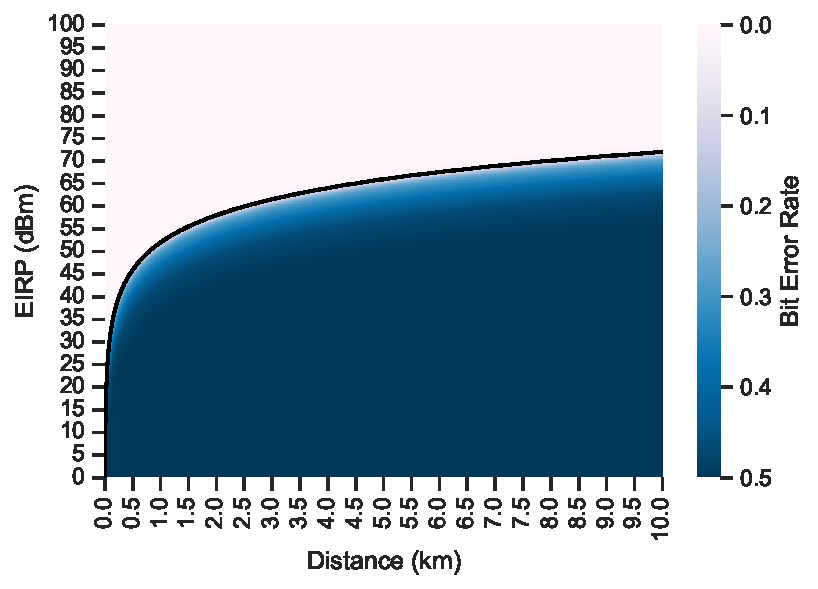
\includegraphics[width=\columnwidth]{diagrams/distance_eirp_heatmap_95.pdf}
    \caption{The bit error rate of the injected signal as the attacker varies EIRP and distance from the receiver. The values beyond which the bit error rate drops below $5$\% are indicated using a line.}
    \label{fig:distance_eirp}
\end{figure}

The first and most obvious countermeasure is to simply encrypt downlinked signals using a cryptographic key known only to the operators, or alternatively to use cryptographic keys to sign the messages.
In both cases this makes it possible to verify that a message is legitimate and has not been tampered with.
If implemented properly, this trivially counteracts the attacks we describe.

However, there are a number of reasons why an organization may decline to use cryptography in an existing system.
We see a large number of existing systems which do not employ cryptographic measures due to the large amounts of computing power required; this is no longer a concern in most newer systems, but can make it difficult to patch existing space systems.
Even in cases where limited computing power is not a concern, the engineering challenges and operational risk of overhauling the communications infrastructure are often considered to outweigh the benefits of the improved security it provides.
Beyond this, it is also considered desirable in some cases for the downlinked data to be openly available to anyone with a suitable receiver.
The EOS data was designed with this in mind, and encrypting the communications would make it more difficult to openly access the data by all the organizations currently relying on it.
Of course, it would still be possible to access the data if it were signed rather than encrypted, but to make this change to an already deployed system would be difficult for the reasons described above.

Further difficulty comes in ensuring its proper implementation; there are a number of difficulties on the path to effective cryptography, and failing to acknowledge these can lead to a system which appears on the surface to be secure but is in reality only marginally better than if no cryptography had been added in the first place.
This provides a false sense of security which is arguably more dangerous than lacking cryptography in the first place, so it is of great importance that we apply the best practices in this area.

The first problem we consider is key management.
Maintaining a single key is certainly the simplest possible system, but all it takes is a single leak for the security of the entire system to be compromised, possibly forever if there is no mechanism for changing keys.
Unlike in terrestrial systems, it is not possible to physically access compromised machines to reset the onboard software or change affected keys.
We see this problem occur in satellites such as GEO-KOMPSAT-2A, the keys to which were leaked with no mechanism to revoke or reset them~\cite{xrit-rx} -- this system is no longer secure and may never be again.
It is much better to build a key management system which supports key issue and revocation to ensure that security can be reestablished in this event.
To verify chain of trust and minimize the risk of compromise, a ``master key'' should be issued which is only used for the purpose of issuing and revoking other keys.

We must also consider management of ``subkeys'' in the case of shared satellite systems.
In these contexts it is not uncommon for different parties to require different levels of access to the data or, in the case of uplinked data, control of the satellite itself.
It is useful in this situation to be able to issue keys with different levels of system access, and for those keys to be able to issue subkeys with a subset of the original key's access.
In the event that a key is revoked, all subkeys must also stop working, so that access can be easily revoked for an entire organization if necessary.
To do so effectively, it is also vital to maintain complete awareness of what keys are currently issued, and therefore which parties have each level of access at any given time.

Finally we must consider the layer at which the cryptographic measures are implemented.
The simplest approach is to simply add these systems to the application layer, requiring only minor changes to the system as a whole.
However, unless sequence numbers are included in the payload of the message this leaves the system wide open to replay attacks.
%\textbf{TODO more here? DoS attacks?}

If instead we implement encryption at a lower layer, all higher-level protocols and applications are secure by default, and replay attacks are prevented thanks to sequence counters baked into the frame header.
Denial-of-service attacks are also mitigated since unencrypted or unsigned messages can be discarded at a much earlier stage than would otherwise be possible.
It is not necessary to design a system that satisfies these conditions from scratch -- the \textit{Space Data Link Security} (SDLS) protocol designed by CCSDS provides support for encryption and authentication on top of the widely-used Space Data Link protocols~\cite{ccsdsSpace2015,ccsdsSpace2020}.
There are free and open-source implementations of these protocols, so they are easy to implement in a newly designed system~\cite{nasaCryptolib}.
SDLS and the associated extended procedures provide mechanisms for message encryption and signature-based authentication, replay protection, maintaining keys for different purposes, and key management (including issue and revocation).
However, it is still the responsibility of the satellite operator to ensure these systems are properly implemented and applied, avoiding use of a single master key for all communication and ensuring access control to core components and data is restricted to all but a few.

In cases where operators have declined to add cryptographic measures to space systems (or are unable to do so), it is important that we consider other methods to mitigate signal injection and overshadowing attacks; the long lifespans and high associated expenses of satellite missions mean we cannot stop using the satellites currently in operation, and must instead find ways to protect them in their current state.
In these cases, we can provide security by observing other properties of the downlinked signal.
All required changes for these are implemented on the ground station, requiring no changes to the space segment of the system -- this provides excellent backwards compatibility with existing systems.


\subsection{Timing Analysis}

The first of these involves assessing the timing of received signals.
This can come in a number of forms, the simplest of which is to ensure that the ground station is not processing signals when the satellite is not passing overhead.
This prevents the attacker from injecting signals at arbitrary times, instead forcing them to wait for a satellite pass.
It does not, however, prevent signal injection entirely.

A more robust form of timing analysis involves measuring Time Difference of Arrival (TDOA) -- that is, comparing the difference between signal arrival times at different sensors to verify the position of the satellite.
This has previously been demonstrated to be a viable method of authenticating satellites~\cite{jedermann2021orbit}.
The position of the satellite is known, so the expected time differences can be computed to verify that the signal has been transmitted from a legitimate source.
If the time differences do not match the expected values to within a certain tolerance, it is likely that the signal has been injected by an attacker at a different location.
The same is true if a signal is received at one location but not another, or if the data received at one location differs from that received at another location.

The difficulty of this method arises from the fact that multiple ground stations are required in order to measure the timing differences.
However, this system is effective and robust, increasing both the effectiveness of measurements and difficulty of overcoming the countermeasure as further sensors are added to the system.
It must also be stated that this does not prevent signal injection attacks entirely; an attacker with transmitters present at each location will be able to compute the expected timing differences and offset their transmission times at each location accordingly.


\subsection{Waveform Analysis}

Alongside looking at the timing of signals, we can also inspect the waveform itself.
This is more difficult than the other proposed countermeasures, as it requires a software-defined radio capable of extracting raw samples from the antenna in addition to the decoded bytes.

If a signal has been overshadowed over a legitimate signal, it will result in a change to the amplitude and SNR of the received signal, as well as possibly creating a momentary shift in the timing of the signal.
A carefully tuned model could measure these values and generate alerts when they change in unexpected ways.
This would provide some amount of confidence that there is currently no signal being injected on top of the legitimate signal, but ultimately provides little real security beyond requiring the attacker to be more precise in their overshadowing.

It may also be possible to analyze the physical properties of the radio signal itself to provide a measure of confidence that the device broadcasting the signal is the one we expect, rather than an attacker-controlled radio transmitter.
Such \textit{fingerprinting} techniques involve learning how the transmitting radio hardware impairs the received signal in a way that is unique to the device and difficult to replicate by all but the most sophisticated radios.
This has been shown to be an effective method of mitigating spoofing attacks by providing an additional method of authenticating the device~\cite{sankheNo2020,oligeri2020past}.


\subsection{Data Inspection}

%Finally, we can assess features specific to the channel coding, data link, or network layer protocols which may be affected as the result of a signal injection.
Finally, we can assess features specific to the data link or network layer protocols, or the underlying data, which may be affected as the result of a signal injection.
This is possibly the simplest of all the countermeasures to implement, as it only requires changes to the software processing pipeline.

In particular we consider general properties of these protocols which we expect to only be violated in adversarial conditions, but not in benign ones.
For instance, random bit-flips, failed checksums, and lossy data are all expected to happen under normal conditions as noise on the data link increases.
However, we do not expect messages to arrive out of order in systems using single-path routing such as TDRSS, so we can take this as an indication that the system may be under attack and alert the system's operators.
Similarly, when the checksum passes we expect all payload data to fulfil certain conditions -- for example, we expect application IDs and instrument numbers to fall within a certain range.
If these conditions do not hold it is likely an attacker is attempting to induce unexpected behavior in the processing system so the data should not be processed.
By adding safety checks such as these we can reduce the risk of exploits caused by malformed input data, and raise the technological bar required for attackers to spoof messages in the first place.

%By looking at features like the sequence numbers of packets, we can detect packets which have been replayed or synthesized by an attacker.
%It is difficult to know the exact sequence numbers which will be used ahead of time, forcing the attacker to modify data in-transit if they want to remain undetected under this method.
%This is of course possible, but it raises the technological bar required which may discourage less motivated attackers.

%We can also assess more variable factors like the bit-error rate to measure unexpected changes which could be the result of an attack, but these are likely to be unreliable due to their variability under changing weather conditions and other factors, and provide little more than another obstacle for the attacker to overcome through better engineering.

Alongside the TDOA analysis techniques already mentioned, we can compare the data received by multiple ground stations (or the data's cryptographic hash) to verify that it has not changed or been tampered with at one location.
This provides a huge amount of robustness, since an attacker must inject signals at a majority of the ground stations for their data to be considered legitimate.
In the case of NASA's EOS fleet, such a system could be achieved by working alongside organizations currently operating their own EOS ground stations to compare data in an automated fashion, providing a significant boost to security at a fairly minor engineering cost.
There are a large number of organizations capable of receiving downlinked EOS signals (168 at the time of writing~\cite{nasaDirect}) spanning the entire globe, so it should be possible to compare signals received by a number of these ground stations to provide improved security for everyone involved.


\subsection{Comparison}

The simpler of each of our timing, waveform, and data analysis techniques are comparable to ``security through obscurity'' -- they provide some measure of assurance against signal tampering, but only in the case where the attacker does not know about the countermeasures' usage.
If we consider an attacker who has full knowledge of the target system, the countermeasures can simply be circumvented by being more careful with signal injection.
However, they are cheap and straightforward to implement, making for a good intermediate response while a more thorough solution is worked on.

On the other hand, data hash comparison, TDOA analysis, and fingerprinting all make signal injection significantly more difficult even in the case where the attacker knows of their existence.
This is particularly clear with hash/TDOA analysis -- an attacker must fool all receivers at multiple physical locations in order to have the same effect on the processing system as before.
The downside is of course that multiple receivers are required, although this should not be an issue for a system like NASA's EOS which already has many ground stations spread around the world.
Waveform analysis techniques may require the installation of new radio hardware capable of extracting raw samples, making their implementation more difficult.
In turn they are more difficult to circumvent, requiring the attacker to perform much more precise overshadowing or to precisely match the fingerprint of the transmitting satellite.

Finally, properly-implemented cryptographic and key management systems remain the best possible solution in the vast majority of cases, where they are possible to implement.
In these systems, the attacker has no hope of successfully fooling the processing system unless keys are leaked.
It is our hope that any new system is built with security first and foremost, using robust encryption or signature systems, and other effective countermeasures are implemented to bolster the security of legacy systems.
By doing so we can verify that the systems and resulting data have not been tampered with and trust the resulting datasets, even as the missions continue into the coming decades.
